\documentclass[t]{beamer}
\usepackage{listings}
\usepackage{minted}
\usepackage{graphicx}
\usetheme{default}

\usebackgroundtemplate{
  
\includegraphics[width=\paperwidth]{../cpeb_bkground_topleftlogo.pdf}}

\setbeamertemplate{frametitle}{
  \centering\vspace{1mm}\insertframetitle\par\vspace{3mm}
}

% \usepackage[style=nature,
%             hyperref,
%             backend=biber,
%             isbn=false,
%             doi=false,
%             url=false,
%             date=year,
%             maxbibnames=3
%            ]{biblatex}
% \bibliography{}

\title{GBS QC and Pipelines}
\author{Kevin Murray}
\institute{Borevitz Lab, CPEB, ANU}
\date{\today}

\usefonttheme{serif}

\begin{document}

{
\usebackgroundtemplate{
\includegraphics[width=\paperwidth]{../cpeb_bkground_centered.pdf}}
\begin{frame}
  \titlepage
  \centering{\small{\textit{``The missing heritablility is in your shitty QC and assembly''}}}
  \vfill
\end{frame}
}

\begin{frame}{The GBS woes}
  \begin{columns}[t]
    \column{0.4\textwidth}
      \begin{itemize}
        \item Reproducibility?
        \item Funky data
        \item Technical Noise
        \item Weird software requirements
        \item Obsolete software?
        \item Weird adaptors or barcodes?
        \item Care to add any?
      \end{itemize}
    \column{0.6\textwidth}
    \begin{figure}[h]
      \centering
      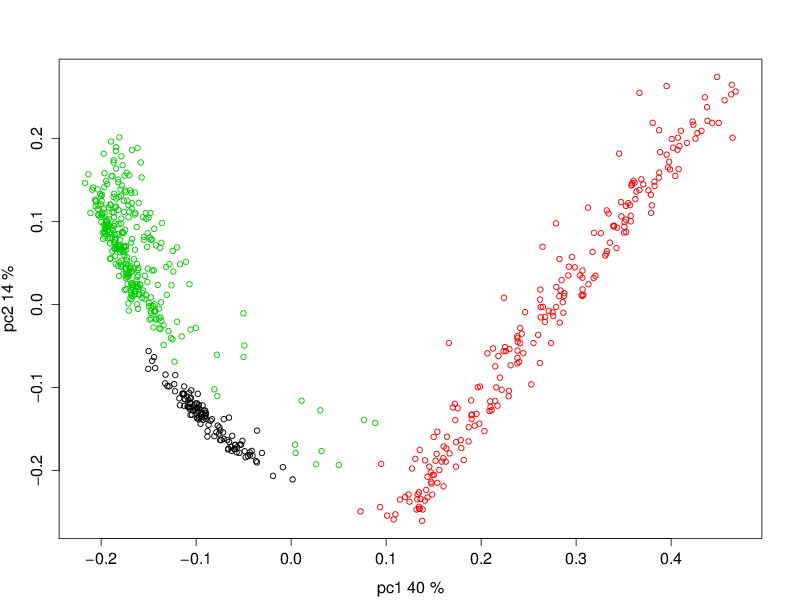
\includegraphics[width=\linewidth]{img/lane-effect.png}
    \end{figure}
  \end{columns}
\end{frame}


% \begin{frame}{The GBS pipeline}
%   \begin{itemize}
%     \item Demultiplex
%     \item Raw QC
%     \item Variant Calling
%     \item SNP QC
%   \end{itemize}
% \end{frame}

\begin{frame}{The GBS pipeline}
  \begin{figure}[h]
    \centering
    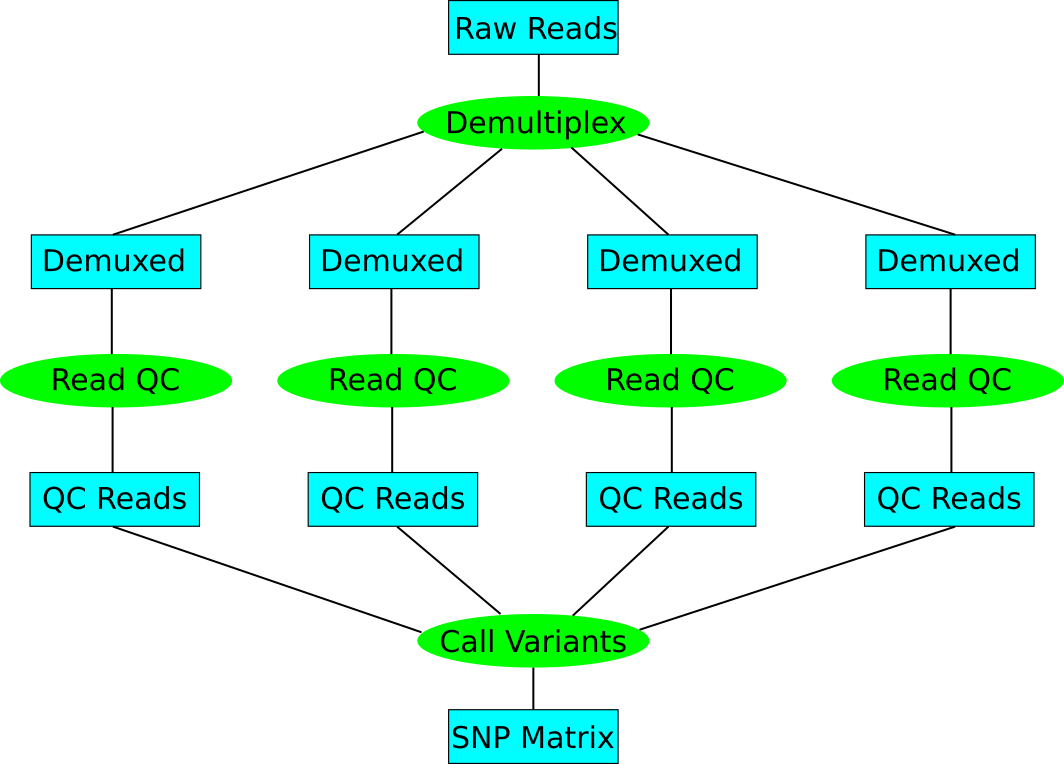
\includegraphics[width=\textwidth]{img/pl-whole.png}
  \end{figure}
\end{frame}

\begin{frame}{Demultiplex}
  \begin{itemize}
    \item Use Axe!
    \item Written in 2014, pretty quick, stable software
    \item Have experiments that show it works (esp. for GBS)
    \item Planning to write it up this year
    \item Now part of the Debian and Ubuntu distributions!
  \end{itemize}
\end{frame}

\begin{frame}{Demultiplex: Practicalities}
  \begin{itemize}
    \item Axe takes a key file per lane
      \begin{itemize}
        \item TSV: Barcode1, Barcode2, samplename
        \item Sample names must be valid paths
        \item Sample names must be unique within lane
      \end{itemize}
    \item (normally) produces 1 interleaved Fastq per sample
    \item Reports stats, saves bad reads to file
  \end{itemize}
  \begin{figure}[h]
    \centering
    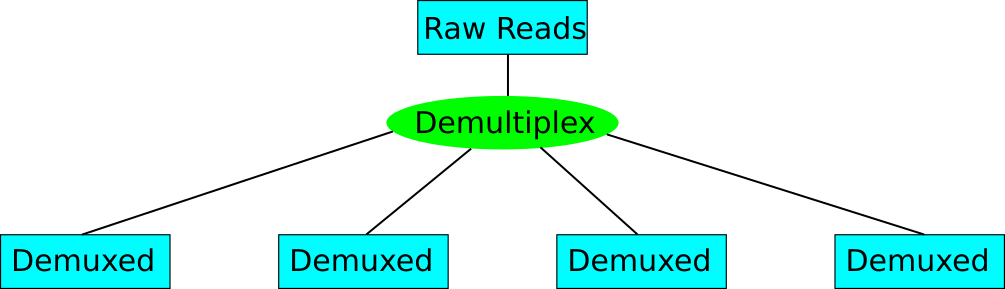
\includegraphics[width=\textwidth]{img/pl-demux.png}
  \end{figure}
\end{frame}

\begin{frame}{GBSQC}
  \begin{columns}[t]
    \column{0.4\textwidth}
    \begin{itemize}
      \item New tool
      \item Written last year, to help Megan \& Jared's data
      \item C++ library and CLI tool
      \item One-stop-shop QC tool
    \end{itemize}
    \column{0.6\textwidth}
    \begin{figure}[h]
      \centering
      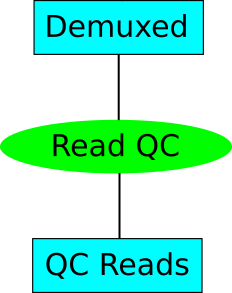
\includegraphics[width=0.5\textwidth]{img/pl-qc-one.png}
    \end{figure}
  \end{columns}
\end{frame}

\begin{frame}{GBSQC}
  \begin{figure}[h]
    \centering
    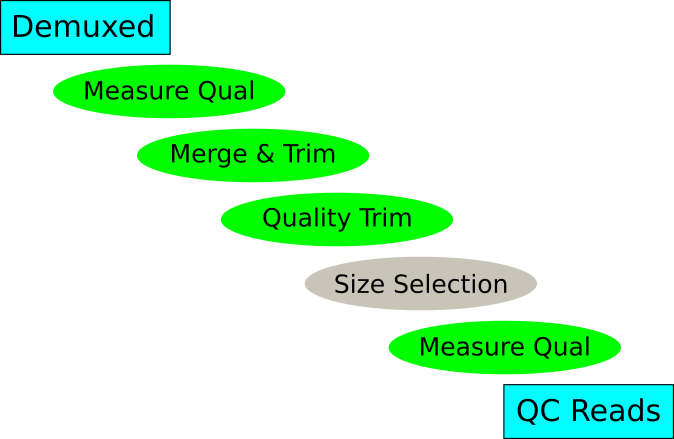
\includegraphics[width=\textwidth]{img/qc.png}
  \end{figure}
\end{frame}

\begin{frame}{TrimMerge}
  \begin{itemize}
    \item Full Needleman-Wunsch Global alignment
    \item Outputs the fragment once if $<190$bp
  \end{itemize}
  \begin{figure}[h]
    \centering
    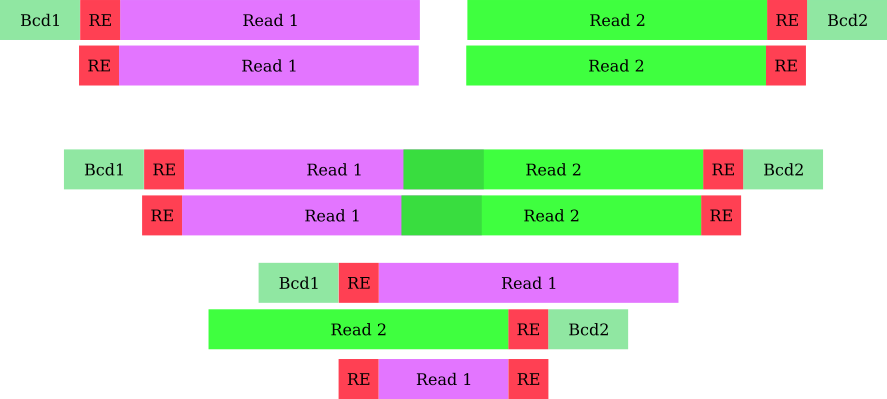
\includegraphics[width=\textwidth]{img/readthru.png}
  \end{figure}
\end{frame}


\begin{frame}{\textit{in silico} Gel Cut}
  \begin{figure}[h]
    \centering
    \includegraphics<1>[width=0.8\linewidth]{img/lane-effect.png}
    \includegraphics<2>[width=0.7\textwidth]{img/size-sel-hist.png}
  \end{figure}
\end{frame}

\begin{frame}{\textit{in silico} Gel Cut}
  \begin{itemize}
    \item Thanks to TrimMerge, we know fragment size
    \item Can digitally select a size range (e.g. 60-150)
    \item Hopefully will help reproducibility
  \end{itemize}
\end{frame}


\begin{frame}{Drinking the Stacks Kool-Aid}
  \begin{itemize}
    \item TASSEL UNEAK
      \begin{itemize}
        \item is deprecated
        \item Seems to to silly things at times
      \end{itemize}
    \item Stacks
      \begin{itemize}
        \item Maintained
        \item New version handels our read types (allegedly)
        \item Seems more efficient computationally
      \end{itemize}
    \item Lets agree to trial stacks for all \textit{de novo} work
  \end{itemize}
\end{frame}

\begin{frame}{Database-automated Demux}
  \begin{itemize}
    \item We have all info need to demux in a DB
    \item We have a somewhat automated QC pipeline
    \item Let's join the two:
      \begin{itemize}
        \item Poll DB for new lanes
        \item Automatically backup to archive
        \item One command to run demux \& QC
        \item Automatically generate Stacks script
        \item Allow independent analysis directory
      \end{itemize}
  \end{itemize}
\end{frame}

\begin{frame}{Slides I didn't get time to write}
  \begin{itemize}
    \item[] {\large But we can talk about now}
    \item Contamination
    \item Database automated demux
    \item Common workflow language pipeline
  \end{itemize}
\end{frame}

\end{document}
